\documentclass[border=6pt]{standalone}
\usepackage{tikz}
% ---- real Helvetica-clone sans-serif (text + math), matching the reference figure ----
\usepackage{tgheros}\renewcommand{\familydefault}{\sfdefault}
\usepackage[T1]{fontenc}
\usepackage{sansmath}
\usetikzlibrary{positioning,fit,backgrounds,calc,arrows.meta,decorations.pathreplacing}
% ---- reference palette: pale fills + matching mid-tone borders, black text ----
\definecolor{txt}{HTML}{000000}
\definecolor{gyF}{HTML}{F2F2F2}\definecolor{gyB}{HTML}{808080}   % grey  (ROM/RTC/radio/SRAM base)
\definecolor{blF}{HTML}{DAE3F3}\definecolor{blB}{HTML}{4472C4}   % blue  (cores)
\definecolor{gnF}{HTML}{E2EFDA}\definecolor{gnB}{HTML}{548235}   % green (flash)
\definecolor{rdF}{HTML}{FBE3E3}\definecolor{rdB}{HTML}{C00000}   % red   (arena highlight)
\definecolor{socB}{HTML}{404040}                                 % SoC boundary
\begin{document}\sansmath
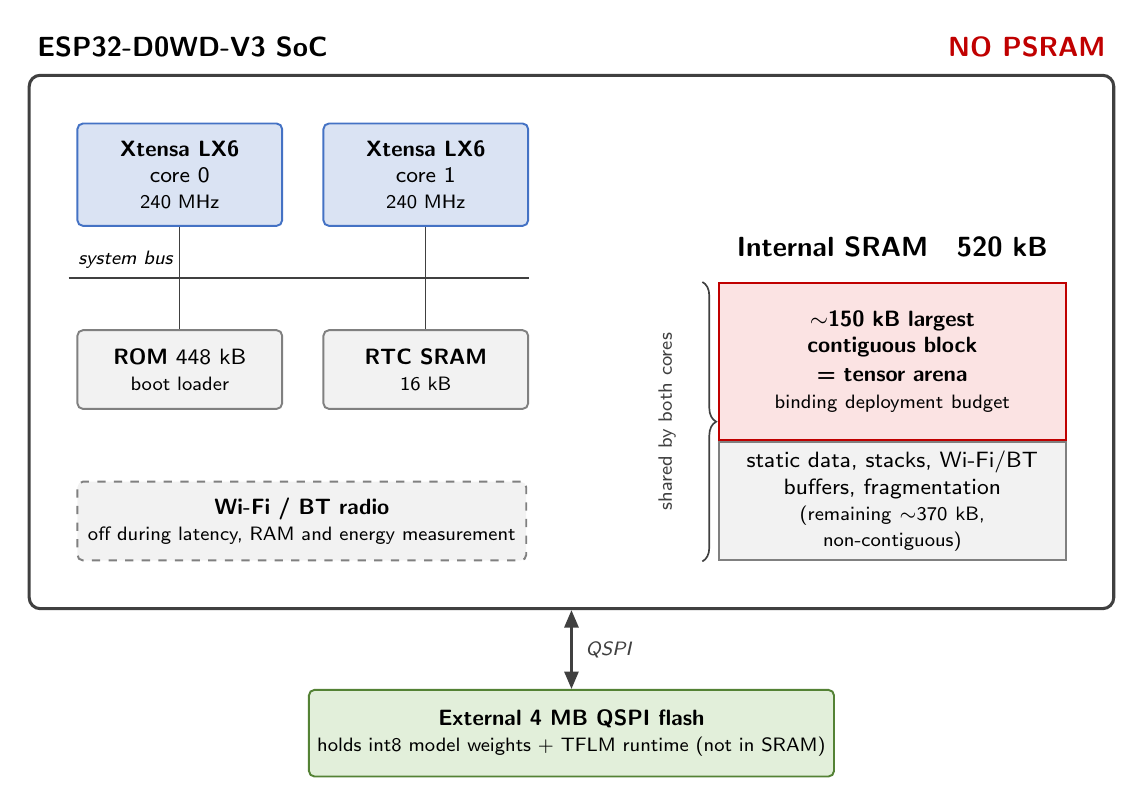
\begin{tikzpicture}[
  font=\footnotesize,text=txt,
  >={Triangle[length=2.2mm,width=1.8mm]},
  bx/.style={rounded corners=2pt,line width=0.7pt,align=center,inner sep=3pt},
  core/.style={bx,fill=blF,draw=blB,minimum width=26mm,minimum height=13mm},
  peri/.style={bx,fill=gyF,draw=gyB,minimum width=26mm,minimum height=10mm},
  seg/.style={line width=0.7pt,minimum width=44mm,text width=40mm,align=center,inner sep=3pt},
  ]

% ================= LEFT: compute + peripherals =================
\node[core] (c0) {\textbf{Xtensa LX6}\\core 0\\\scriptsize 240 MHz};
\node[core,right=5mm of c0] (c1) {\textbf{Xtensa LX6}\\core 1\\\scriptsize 240 MHz};

\node[peri,below=13mm of c0] (rom) {\textbf{ROM} 448 kB\\\scriptsize boot loader};
\node[peri,below=13mm of c1] (rtc) {\textbf{RTC SRAM}\\\scriptsize 16 kB};

\node[peri,dashed,minimum width=57mm,below=9mm of rom.south west,anchor=north west]
  (radio) {\textbf{Wi-Fi / BT radio}\\\scriptsize off during latency, RAM and energy measurement};

% ---- system bus rail (between cores and peripherals) ----
\coordinate (busL) at ($(c0.south west)!0.5!(rom.north west)+(-1mm,0)$);
\coordinate (busR) at (busL-|c1.east);
\draw[line width=1pt,socB] (busL) -- (busR);
\node[anchor=south west,font=\scriptsize\itshape] at (busL) {system bus};
\foreach \n in {c0,c1}{\draw[socB,line width=0.5pt] (\n.south) -- (\n.south|-busL);}
\foreach \n in {rom,rtc}{\draw[socB,line width=0.5pt] (\n.north) -- (\n.north|-busL);}

% ================= RIGHT: the memory budget =================
\node[seg,fill=gyF,draw=gyB,minimum height=15mm,anchor=south west] (s_res)
  at ([xshift=24mm]c1.north east |- radio.south) {static data, stacks, \mbox{Wi-Fi/BT} buffers, fragmentation\\\scriptsize (remaining \mbox{$\sim$370 kB}, non-contiguous)};
\node[seg,fill=rdF,draw=rdB,minimum height=20mm,above=0pt of s_res] (s_arena)
  {\textbf{$\sim$150 kB largest contiguous block}\\[1pt]\textbf{= tensor arena}\\\scriptsize binding deployment budget};

\node[anchor=south,font=\bfseries] at ([yshift=2mm]s_arena.north) {Internal SRAM \; 520 kB};
\draw[decorate,decoration={brace,amplitude=5pt},socB,line width=0.6pt]
  ([xshift=-2mm]s_arena.north west) -- ([xshift=-2mm]s_res.south west)
  node[midway,left=6pt,font=\scriptsize,align=center,rotate=90,anchor=south]{shared by both cores};

% ================= SoC boundary =================
\begin{scope}[on background layer]
\node[draw=socB,line width=1.1pt,rounded corners=4pt,
      fit=(c0)(c1)(rom)(rtc)(radio)(s_res)(s_arena),inner sep=6mm] (soc) {};
\end{scope}
\node[anchor=south west,font=\bfseries] at ([yshift=1mm]soc.north west) {ESP32-D0WD-V3 SoC};
\node[anchor=south east,font=\bfseries,text=rdB] at ([yshift=1mm]soc.north east) {NO PSRAM};

% ================= External flash =================
\node[bx,fill=gnF,draw=gnB,minimum width=57mm,minimum height=11mm,below=10mm of soc.south]
  (fl) {\textbf{External 4 MB QSPI flash}\\\scriptsize holds int8 model weights + TFLM runtime (not in SRAM)};
\draw[<->,line width=0.8pt,socB] (soc.south) -- (fl.north)
  node[midway,right=0.5mm,font=\scriptsize\itshape]{QSPI};

\end{tikzpicture}
\end{document}
